\section{Auswertung}
\subsection{Die Drillachse}
\subsubsection{Die Winkelrichtgröße}\label{subsubsec:D}
Um die Winkelrichtgröße $D$ der Drillachse zu bestimmen wird Gleichung
\eqref{eq:D}
verwendet. Die Ergebnisse werden über die Formel für den Mittelwert
\[\bar{D}=\frac{1}{N}\sum_{i=1}^ND_.i\] 
gemittelt und für die Bestimmung der Standardabweichung wird die Formel 
\[\sigma_.D=\sqrt{\frac{1}{N(N-1)}\sum_{i=1}^N(D_.i-\bar{D})^2}\]
verwendet.\newline
Die benötigten Werte für die Kraft $F$, den Radius $r$ und den Winkel $\phi$, sowie die zugehörigen Werte für $D$ lassen sich der Tabelle \ref{tab:tab1}
entnehmen.
\[\bar{D}=\SI{2,56(6)e-2}{\joule}\]
\begin{table}
	\centering
	\caption{Messdaten zur Winkelrichtgrößenbestimmung}
	\sisetup{table-format=1.2}
	\begin{tabular}{S[table-format=3.2] S[table-format=3.2]S[table-format=3.2]S[table-format=3.2]}
		\toprule
		{$F/\si[per-mode=reciprocal]{\newton}$}&{$r/\si[per-mode=reciprocal]{\metre}$}&{$\phi/\si[per-mode=reciprocal]{\radian}$}&{$D/\si[per-mode=reciprocal]{\joule}$} \\
		\midrule
		0,12 & 0,119 & 0,524 & 0,0273 \\
		0,19 & 0,119 & 0,873 & 0,0259 \\		
		0,38 & 0,059 & 0,873 & 0,0257 \\
		0,16 & 0,190 & 1,047 & 0,0290 \\
		0,20 & 0,170 & 1,222 & 0,0278 \\
		0,30 & 0,110 & 1,396 & 0,0236 \\
		0,28 & 0,139 & 1,571 & 0,0248 \\
		0,27 & 0,159 & 1,745 & 0,0246 \\
		0,30 & 0,170 & 2,094 & 0,0243 \\
		0,22 & 0,239 & 2,269 & 0,0232 \\
		\bottomrule
	\end{tabular}
	\label{tab:tab1}
\end{table}
\subsubsection{Eigenträgheitsmoment}\label{subsubsec:I_D}
Zur Bestimmung des Eigenträgheitsmoments werden zwei Zylinder mit dem Durchmesser $d = \SI{0,035}{\metre}$, der Höhe $h = \SI{0,03}{\metre}$ und der Masse $m = \SI{0,2218}{\kilogram}$ benutzt.\newline Die Verbindungsstange wird als masselos angenommen und wird daher nicht berücksichtigt.
Die Werte für das Quadrat der Periodendauer $T$ und des Abstands $a$ aus Tabelle \ref{tab:tab2} sind im Graph \ref{fig:abb2} gegeneinander aufgetragen. Mittels der linearer Regression $f(x) = m \cdot x + n$\cite{matplotlib}, ergibt sich hier als Achsenabschnitt \[T_.0^2=\SI{5,0(2)}{\second\squared}\]
Mit Gleichung \eqref{eq:I_D} ergibt sich für das Trägheitsmoment $I_.D$ der Drillachse:
\[I_.D=\SI{3,2(1)e-3}{\kilogram\metre\squared}\]
Die Messungenauigkeit ergibt sich dabei aus der Formel der Gaußschen Fehlerfortpflanzung
\[\sigma_.{I_.D}= \sqrt{(\frac{\mathrm{d}(I_.D)}{\mathrm{d}(T^2_.0)} \cdot \sigma_.{T^2_.0})^2+(\frac{\mathrm{d}(I_.D)}{\mathrm{d}D}\cdot\sigma_.D)^2},\]
wobei $\sigma_.{T^2_.0}$ der Fehler des Achsenabschnitts und $\sigma_.D$ aus Abschnitt \ref{subsubsec:D} bekannt ist.
\begin{figure}
\centering
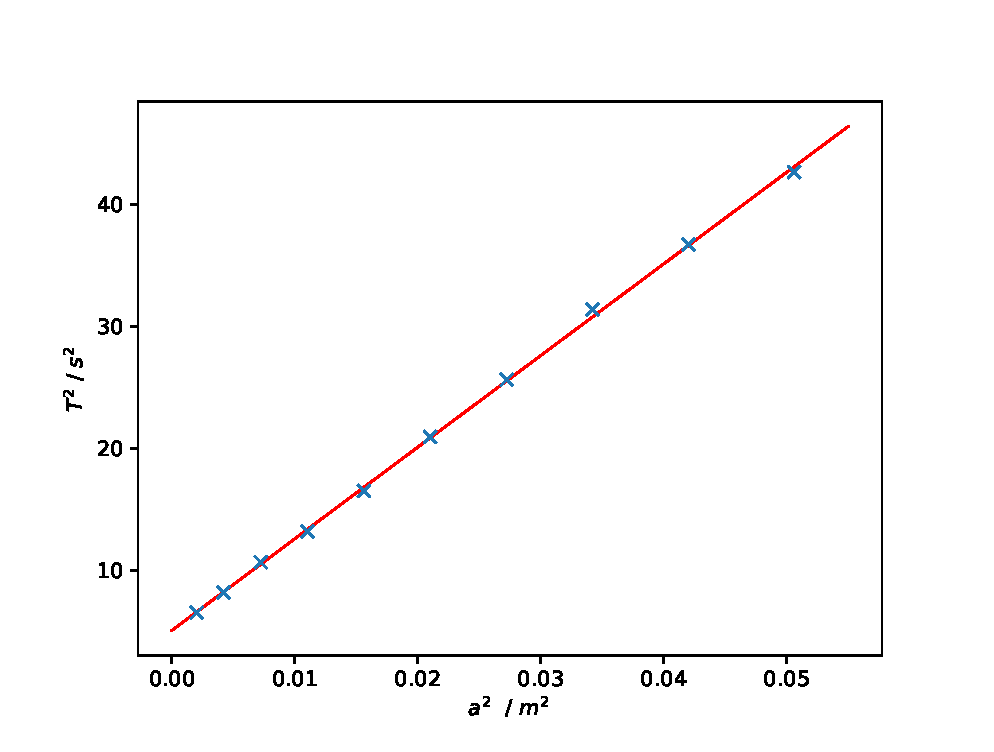
\includegraphics[scale = .75,keepaspectratio]
	{content/images/plot1.eps}
\caption{Graph der Messdaten zur Bestimmung des Eigenträgheitsmoments der Drillachse}\label{fig:abb2}
\end{figure}
\begin{table}
	\centering
	\caption{Messdaten zur Eigenträgheitsmomentbestimmung}
	\sisetup{table-format=1.2}
	\begin{tabular}{S[table-format=3.2] S[table-format=3.2]S[table-format=3.2]S[table-format=3.2]}
		\toprule
		{$a/\si[per-mode=reciprocal]{\metre}$}&{$T_.4/\si[per-mode=reciprocal]{\second}$}&{$T/\si[per-mode=reciprocal]{\second}$} \\
		\midrule
		0,045 & 10,21 & 2,5525 \\
		0,065 & 11,44 & 2,86 \\
		0,085 & 13,07 & 3,2675 \\
		0,105 & 14,52 & 3,63 \\
		0,125 & 16,26 & 4,065 \\
		0,145 & 18,30 & 4,575 \\
		0,165 & 20,24 & 5,06 \\
		0,185 & 22,40 & 5,60 \\
		0,205 & 24,24 & 6,06 \\
		0,225 & 26,12 & 6,53 \\
		\bottomrule
	\end{tabular}
	\label{tab:tab2}
\end{table}

\subsection{Das Trägheitsmomentmoment einer Kugel}
\begin{table}
	\centering
	\caption{Messdaten zur Trägheitsmomentbestimmung einer Kugel}
	\sisetup{table-format=1.2}
	\begin{tabular}{S[table-format=3.2] S[table-format=3.2]S[table-format=3.2]S[table-format=3.2]}
		\toprule
		{$T_.{mess}/\si[per-mode=reciprocal]{\second}$} & {$T_.1/\si[per-mode=reciprocal]{\second}$} \\
		\midrule
		6,87 & 1,7175 \\
		6,89 & 1,7225 \\
		6,90 & 1,7250 \\
		6,89 & 1,7225 \\
		7,55 & 1,5100 \\
		\bottomrule
	\end{tabular}
	\label{tab:tab3}
\end{table}
\noindent Das Trägheitsmoment einer Kugel bestimmt sich nach Gleichung \eqref{eq:I_K}.
Die Werte für die Periodendauer $T_.1$ lassen sich dabei aus Tabelle \ref{tab:tab3} entnehmen. Dabei entsprechen die ersten vier Werte von $T_.{mess}$ vier Periodendauern und der letzte fünf Perioden.
Der Fehler errechnet sich dabei über
\[\sigma_.{I_.{Kugel}}= \sqrt{(\frac{\mathrm{d}(I_.K)}{\mathrm{d}(T^2_.0)} \cdot \sigma_.{T^2_.0})^2+(\frac{\mathrm{d}(I_.K)}{\mathrm{d}D}\cdot\sigma_.D)^2}(\frac{\mathrm{d}(I_.K)}{\mathrm{d}(I_.D)} \cdot \sigma_.{I_.D})^2,\]
wobei sich die Messungenauigkeit $\sigma_.{T^2_.0}$ aus der Formel für die Standardabweichung
\[\sigma_.x=\sqrt{\frac{1}{N(N-1)}\sum_{i=1}^N(x_.i-\bar{x})^2}\text{.}\]
$\sigma_.{D}$ und $\sigma_.{I_.D}$ sind bereits aus Abschnitt \ref{subsubsec:D} und \ref{subsubsec:I_D} bekannt.
Damit ist
\[I_.{Kugel}=\SI{-1,4(2)e-3}{\kilogram\metre\squared}\]
Die Kugel besitzt die Masse $m=\SI{0,8124}{\kilogram}$ und den Durchmesser $d=2R=\SI{0,1374}{\metre}$.
Daraus ergibt sich der Theoriewert nach Formel \eqref{eq:I_SK}
zu
\[I_.{Kugel,Theorie}=\SI{1,5e-3}{\kilogram\metre\squared}\]

\subsection{Das Trägheitsmoment eines Zylinders}
\begin{table}
	\centering
	\caption{Messdaten zur Trägheitsmomentbestimmung eines Zylinders}
	\sisetup{table-format=1.2}
	\begin{tabular}{S[table-format=3.2] S[table-format=3.2]S[table-format=3.2]S[table-format=3.2]}
		\toprule
		{$T_.4/\si[per-mode=reciprocal]{\second}$} & {$T_.1/\si[per-mode=reciprocal]{\second}$} \\
		\midrule
		4.69 & 1,1725 \\
		4.76 & 1,1900 \\
		4.64 & 1,1600 \\
		4.66 & 1,1650 \\
		4.73 & 1,1825 \\
		\bottomrule
	\end{tabular}
	\label{tab:tab4}
\end{table}
Das Trägheitsmoment eines Zylinders berechnet sich nach Gleichung \eqref{eq:I_K}.
Die Werte für die Periodendauer $T$ lassen sich dabei aus Tabelle \ref{tab:tab4} entnehmen:
\[I_.{Zylinder}=\SI{-2,33(2)e-3}{\kilogram\metre\squared}\]
Der Fehler errechnet sich dabei über
\[\sigma_.{I_.{Zylinder}}= \sqrt{(\frac{\mathrm{d}(I_.K)}{\mathrm{d}(T^2_.0)} \cdot \sigma_.{T^2_.0})^2+(\frac{\mathrm{d}(I_.K)}{\mathrm{d}D}\cdot\sigma_.D)^2}(\frac{\mathrm{d}(I_.K)}{\mathrm{d}(I_.D)} \cdot \sigma_.{I_.D})^2,\]
wobei sich die Messungenauigkeit $\sigma_.{T^2_.0}$ aus der Formel für die Standardabweichung
\[\sigma_.x=\sqrt{\frac{1}{N(N-1)}\sum_{i=1}^N(x_.i-\bar{x})^2}\text{.}\]
$\sigma_.{D}$ und $\sigma_.{I_.D}$ sind bereits aus Abschnitt \ref{subsubsec:D} und \ref{subsubsec:I_D} bekannt.
Der Zylinder besitzt die Masse $m = \SI{1,1193}{\kilogram}$, den Durchmesser 
$d = 2R = \SI{0,0751}{\metre}$ und die Höhe $h = \SI{0,03}{\metre}$
Damit ergibt sich der Theoriewert für einen Zylinder dessen Körperachse identisch mit der Drehachse ist nach Formel \eqref{eq:I_SZ}
beträgt:
\[I_.{Zylinder,Theorie}=\SI{7,9e-4}{\kilogram\metre\squared}\]
\subsection{Trägheitsmomente einer Puppe}
Da nur die Gesamtmasse der Puppe gemessen werden kann ($m_.P=\SI{0,3395}{\kilogram}$ und die Puppe näherungsweise in einfache geometrische Figuren zerlegt werden kann, wird bei der Ermittlung des Theoriewertes über das Verhältnis der Einzelvolumina zum Gesamtvolumen die Masse der jeweiligen Körper berechnet. 
Der Kopf wird als Kugel und Arme, Beine und Rumpf als Zylinder genähert.
Die Masse $m$ der Durchmesser $d$ und die Höhe $h$ lassen sich aus Tabelle \ref{tab:tab5} ablesen.
\begin{table}
	\centering
	\caption{Abmessungen der Puppe}
	\sisetup{table-format=1.2}
	\begin{tabular}{cS[table-format=3.2]S[table-format=3.2]S[table-format=3.2]}
		\toprule
		{}&{$d/\si[per-mode=reciprocal]{\metre}$}&{$h/\si[per-mode=reciprocal]{\metre}$}&{$V/\si[per-mode=reciprocal]{\metre\cubic}$}&{$m/\si[per-mode=reciprocal]{\kilo\gram}$} \\
		\midrule
		Arme & 0,018 & 0,180 & 0,000093 & 0,062 \\
		Beine & 0,023 & 0,198 & 0,000166 & 0,110 \\
		Rumpf & 0,048 & 0,125 & 0,000226 & 0,151 \\
		Kopf  & 0,036 & & 0,000025 & 0,017 \\
		\bottomrule
	\end{tabular}
	\label{tab:tab5}
\end{table}
\subsubsection{Puppe mit ausgebreiteten Armen und geschlossenen Beinen}
\begin{table}
	\centering
	\caption{Messdaten zur Periodendauer einer Puppe mit ausgebreiteten Armen}
	\sisetup{table-format=1.2}
	\begin{tabular}{S[table-format=3.2] S[table-format=3.2]S[table-format=3.2]S[table-format=3.2]}
		\toprule
		{$T_.4/\si[per-mode=reciprocal]{\second}$} &{$T_.1/\si[per-mode=reciprocal]{\second}$} \\
		\midrule
		5,09 & 1,2725 \\
		5,12 & 1,2800 \\
		5,00 & 1,2500 \\
		5,07 & 1,2675 \\
		5,03 & 1,2575 \\
		\bottomrule
	\end{tabular}
	\label{tab:tab6}
\end{table}
\noindent Aus Formel \eqref{eq:I_K} folgt mit den Werten für die Periodendauer $T_.1$ aus Tabelle \ref{tab:tab6}
berechnen:
\[I_.{Puppe,ausg}=\SI{-2,18(13)e-3}{\kilo\gram\metre\squared}\]
Der Fehler errechnet sich dabei über
\[\sigma_.{I_.{Puppe,ausg}}= \sqrt{(\frac{\mathrm{d}(I_.K)}{\mathrm{d}(T^2_.0)} \cdot \sigma_.{T^2_.0})^2+(\frac{\mathrm{d}(I_.K)}{\mathrm{d}D}\cdot\sigma_.D)^2}(\frac{\mathrm{d}(I_.K)}{\mathrm{d}(I_.D)} \cdot \sigma_.{I_.D})^2,\]
wobei sich die Messungenauigkeit $\sigma_.{T^2_.0}$ aus der Formel für die Standardabweichung
\[\sigma_.x=\sqrt{\frac{1}{N(N-1)}\sum_{i=1}^N(x_.i-\bar{x})^2}\text{.}\]
$\sigma_.{D}$ und $\sigma_.{I_.D}$ sind bereits aus Abschnitt \ref{subsubsec:D} und \ref{subsubsec:I_D} bekannt.
Der genäherte Theoriewert berechnet sich durch Gleichung \eqref{eq:I_S} und mit dem Satz von Steiner zu 
\[I_.{Puppe,aus,theo}\approx\SI{2,07e-3}{\kilo\gram\metre\squared}\]
\subsubsection{Puppe mit angelegten Armen und geschlossenen Beinen}
\begin{table}
	\centering
	\caption{Messdaten zur Periodendauer einer Puppe mit angelegten Armen}
	\sisetup{table-format=1.2}
	\begin{tabular}{S[table-format=3.2] S[table-format=3.2]S[table-format=3.2]S[table-format=3.2]}
		\toprule
		{$T_.4/\si[per-mode=reciprocal]{\second}$} &{$T_.1/\si[per-mode=reciprocal]{\second}$} \\
		\midrule
		3.55 & 0,8875 \\
		3.58 & 0,8950 \\
		3.56 & 0,8900 \\
		3.55 & 0,8875 \\
		3.53 & 0,8825 \\
		\bottomrule
	\end{tabular}
	\label{tab:tab7}
\end{table}
\noindent Aus Formel \eqref{eq:I_K} ergibt sich mit den Werten für die Periodendauer$T_.1$ aus Tabelle \ref{tab:tab7}:
\[I_.{Puppe,ang}=\SI{-2,71(1)e-3}{\kilo\gram\metre\squared}\]
Der Fehler errechnet sich dabei über
\[\sigma_.{I_.{Puppe,ang}}= \sqrt{(\frac{\mathrm{d}(I_.K)}{\mathrm{d}(T^2_.0)} \cdot \sigma_.{T^2_.0})^2+(\frac{\mathrm{d}(I_.K)}{\mathrm{d}D}\cdot\sigma_.D)^2}(\frac{\mathrm{d}(I_.K)}{\mathrm{d}(I_.D)} \cdot \sigma_.{I_.D})^2,\]
wobei sich die Messungenauigkeit $\sigma_.{T^2_.0}$ aus der Formel für die Standardabweichung
\[\sigma_.x=\sqrt{\frac{1}{N(N-1)}\sum_{i=1}^N(x_.i-\bar{x})^2}\text{.}\]
$\sigma_.{D}$ und $\sigma_.{I_.D}$ sind bereits aus Abschnitt \ref{subsubsec:D} und \ref{subsubsec:I_D} bekannt.
Der genäherten Theoriewert berechnet sich durch Gleichung \eqref{eq:I_S} und mit dem Satz von Steiner zu
\[I_.{Puppe,an,theo} \approx \SI{1,52e-4}{\kilo\gram\metre\squared} \]